\chapter{The Internet}

\section*{Overview}
The Internet is a global network of interconnected computer networks that use standardized communication protocols. This unit covers core concepts about how the Internet works and its impact on society.

\section{Internet Architecture}
\begin{itemize}
    \item \textbf{Devices}: Computers, routers, switches, and servers
    \item \textbf{Packets}: Small units of data that travel across networks
    \item \textbf{Bandwidth}: Maximum data transfer rate of a network
\end{itemize}

\begin{figure}[h]
    \centering
    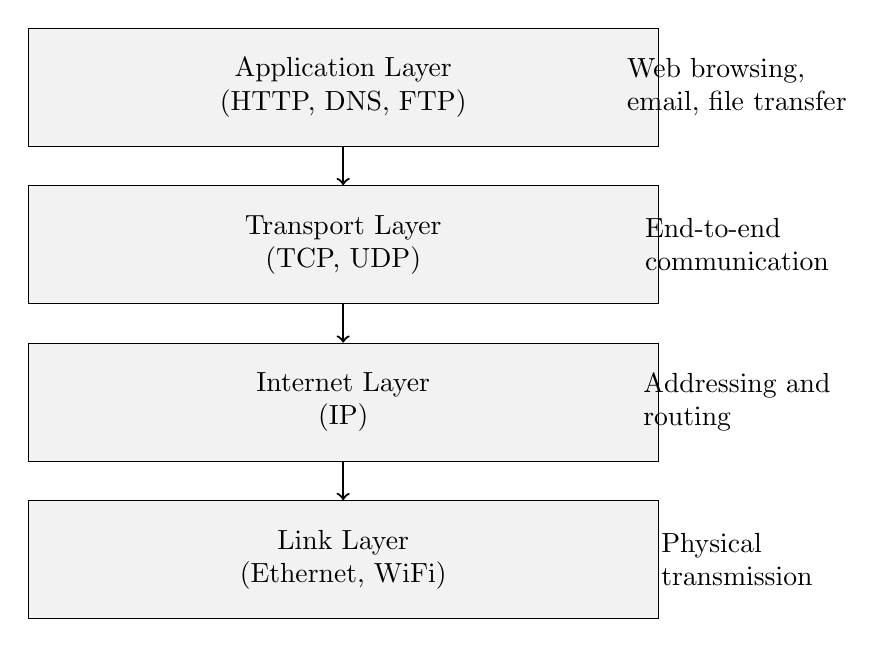
\begin{tikzpicture}[
        box/.style={
            draw,
            rectangle,
            minimum width=8cm,
            minimum height=1.5cm,
            text width=7.5cm,
            align=center,
            fill=gray!10
        }
    ]
        % Layer boxes
        \node[box] (app) at (0,6) {Application Layer\\(HTTP, DNS, FTP)};
        \node[box] (transport) at (0,4) {Transport Layer\\(TCP, UDP)};
        \node[box] (internet) at (0,2) {Internet Layer\\(IP)};
        \node[box] (link) at (0,0) {Link Layer\\(Ethernet, WiFi)};
        
        % Arrows between layers
        \draw[->,thick] (app.south) -- (transport.north);
        \draw[->,thick] (transport.south) -- (internet.north);
        \draw[->,thick] (internet.south) -- (link.north);
        
        % Add labels on the right
        \node[align=left] at (5,6) {Web browsing,\\email, file transfer};
        \node[align=left] at (5,4) {End-to-end\\communication};
        \node[align=left] at (5,2) {Addressing and\\routing};
        \node[align=left] at (5,0) {Physical\\transmission};
        
    \end{tikzpicture}
    \caption{The four layers of the Internet protocol suite}
    \label{fig:network-layers}
\end{figure}

\section{Protocols}
\begin{itemize}
    \item \textbf{TCP/IP}: Core protocols for reliable data transmission
    \item \textbf{HTTP/HTTPS}: Web communication protocols
    \item \textbf{DNS}: Domain Name System for converting URLs to IP addresses
\end{itemize}

\section{Addressing and Routing}
\begin{itemize}
    \item \textbf{IP Addresses}: Unique identifiers for devices (IPv4, IPv6)
    \item \textbf{Routing}: How data finds its path across networks
    \item \textbf{Domain Names}: Human-readable web addresses
\end{itemize}

\section{Cybersecurity}
\begin{itemize}
    \item \textbf{Common Threats}:
        \begin{itemize}
            \item Phishing: Deceptive attempts to steal user data
            \item DDoS: Distributed Denial of Service attacks
            \item Malware: Malicious software types
        \end{itemize}
    \item \textbf{Protection Methods}:
        \begin{itemize}
            \item Encryption: Securing data transmission
            \item Authentication: Verifying user identity
            \item Updates: Maintaining system security
        \end{itemize}
\end{itemize}

\section{Impact on Society}
\begin{itemize}
    \item \textbf{Digital Divide}: Inequality in Internet access
    \item \textbf{Privacy Concerns}: Data collection and surveillance
    \item \textbf{Innovation}: Economic and technological advancement
\end{itemize}